\chapter{Analysis of Feed Architectures}\label{appendix:feed-architecture-analysis}

\begin{figure}[htbp]
    \centering

    \begin{minipage}{0.5\textwidth}
        \centering
        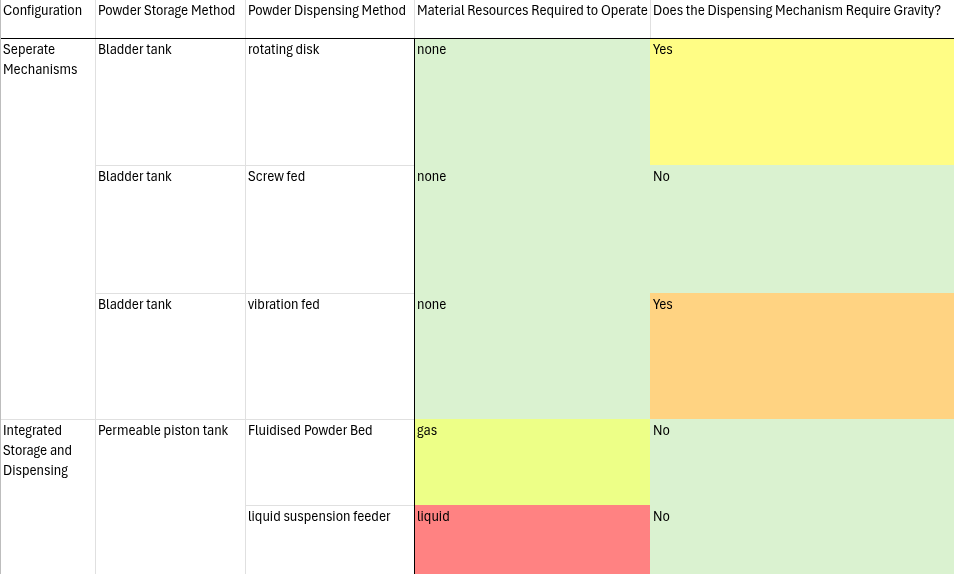
\includegraphics[width=\textwidth]{../report_assets/table_comp_1_1.png}
        \caption{(a) Start}
    \end{minipage}
    \begin{minipage}{0.5\textwidth}
        \centering
        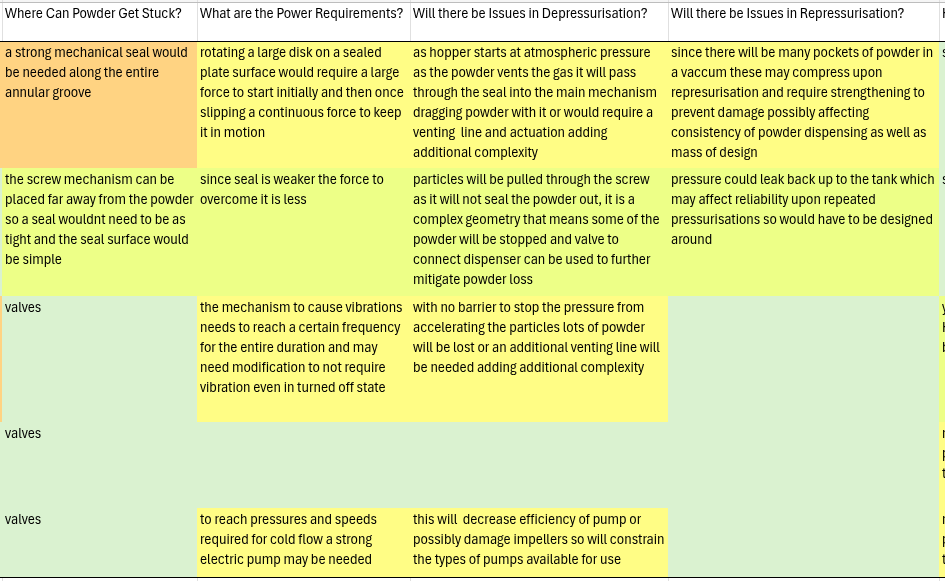
\includegraphics[width=\textwidth]{../report_assets/table_comp_1_2.png}
        \caption{(b) Middle}
    \end{minipage}
    \begin{minipage}{0.5\textwidth}
        \centering
        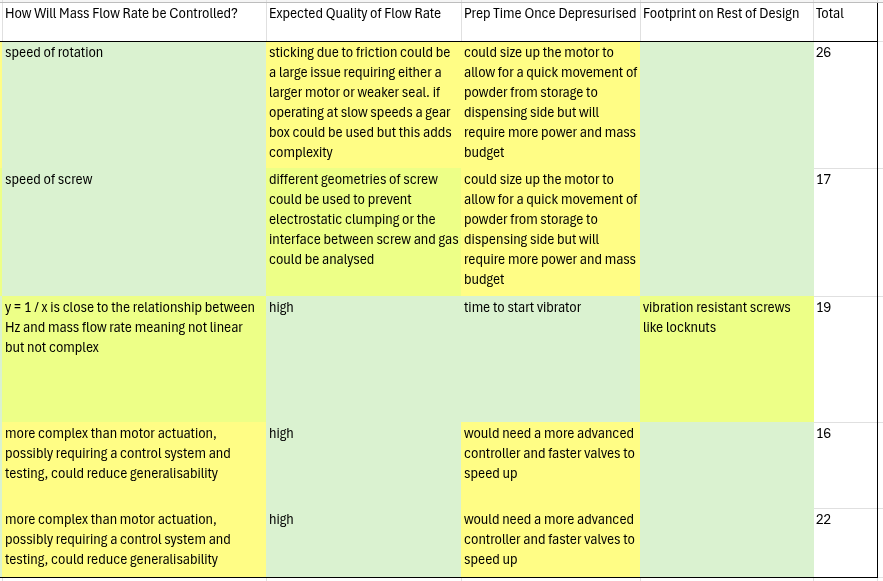
\includegraphics[width=\textwidth]{../report_assets/table_comp_1_3.png}
        \caption{(c) End}
    \end{minipage}
    \caption{Comparison of Suitability of Design Paradigm Unedited}
\end{figure}

\begin{figure}[htbp]
    \centering

    \begin{minipage}{0.5\textwidth}
        \centering
        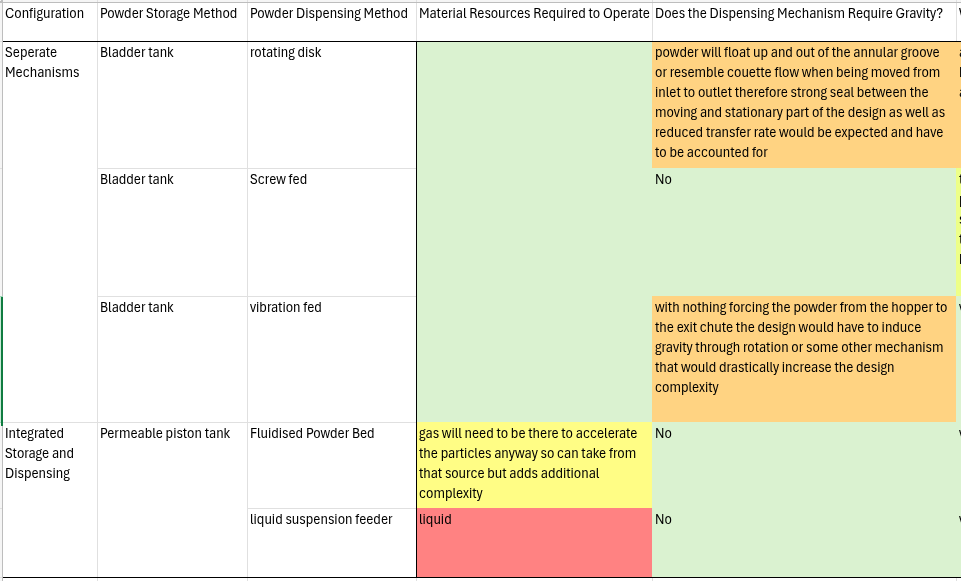
\includegraphics[width=\textwidth]{../report_assets/table_comp_2_1.png}
        \caption{(a) Start}
    \end{minipage}
    \begin{minipage}{0.5\textwidth}
        \centering
        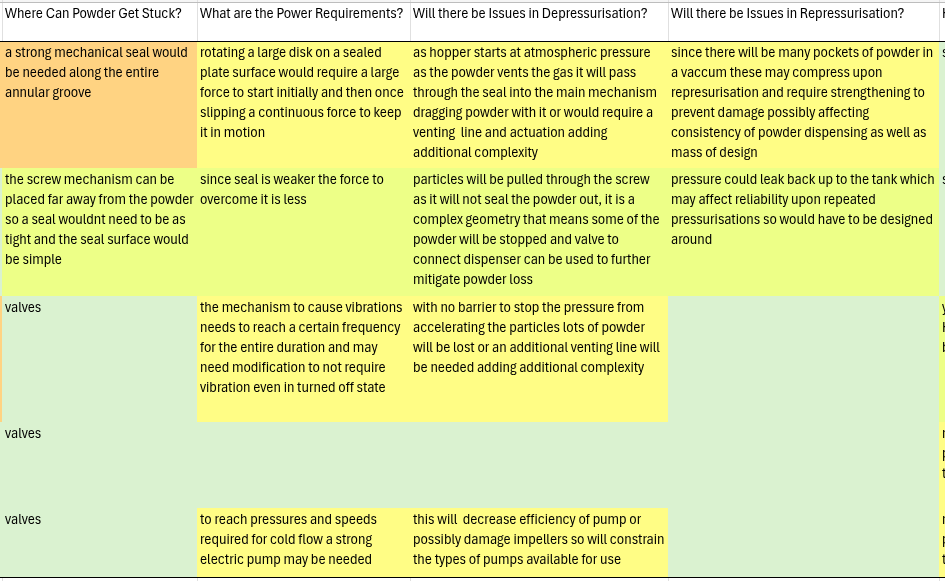
\includegraphics[width=\textwidth]{../report_assets/table_comp_2_2.png}
        \caption{(b) Middle}
    \end{minipage}
    \begin{minipage}{0.5\textwidth}
        \centering
        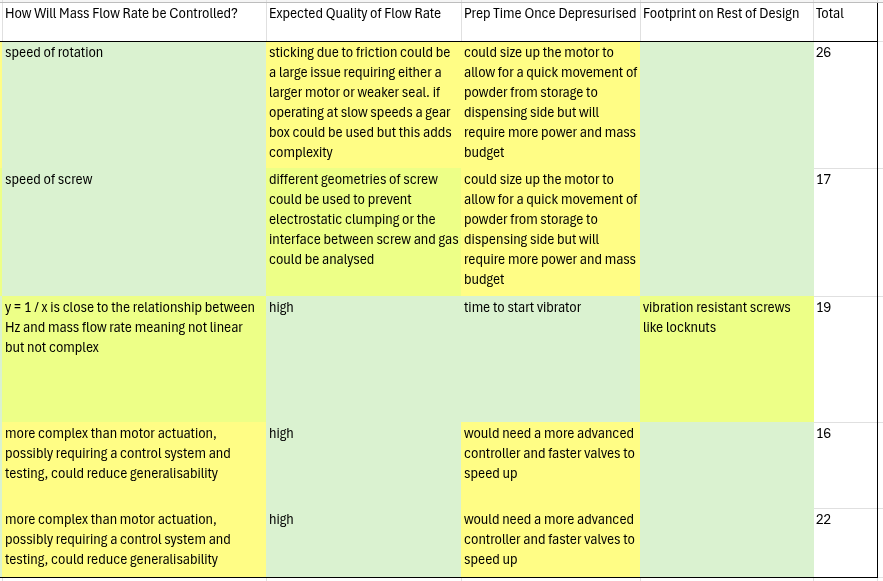
\includegraphics[width=\textwidth]{../report_assets/table_comp_2_3.png}
        \caption{(c) End}
    \end{minipage}
    \caption{Comparison of Difficulty of Edits Required}
\end{figure}

\chapter{Unprocessed Simulation Images}\label{sec:unprocessed-images}
As the images in \autoref{sec:prev-design-analysis} are heavily processed, the unprocessed ones are provided here for clarity.
\begin{figure}[htbp]
    \centering

    \begin{minipage}{0.45\textwidth}
        \centering
        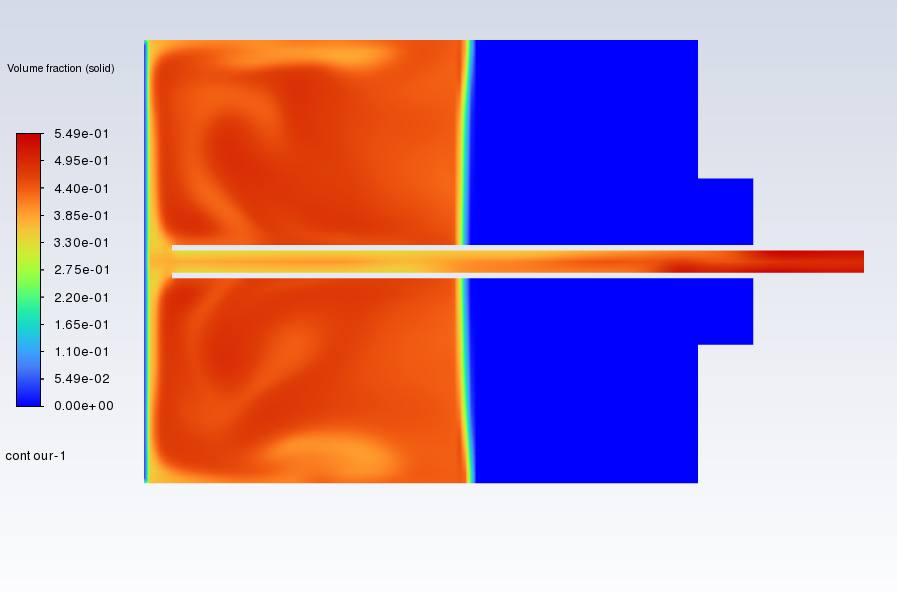
\includegraphics[width=\textwidth]{../report_assets/grav.png}
        \caption*{(a) Under Earth's Gravity}
    \end{minipage}
    \hfill
    \begin{minipage}{0.45\textwidth}
        \centering
        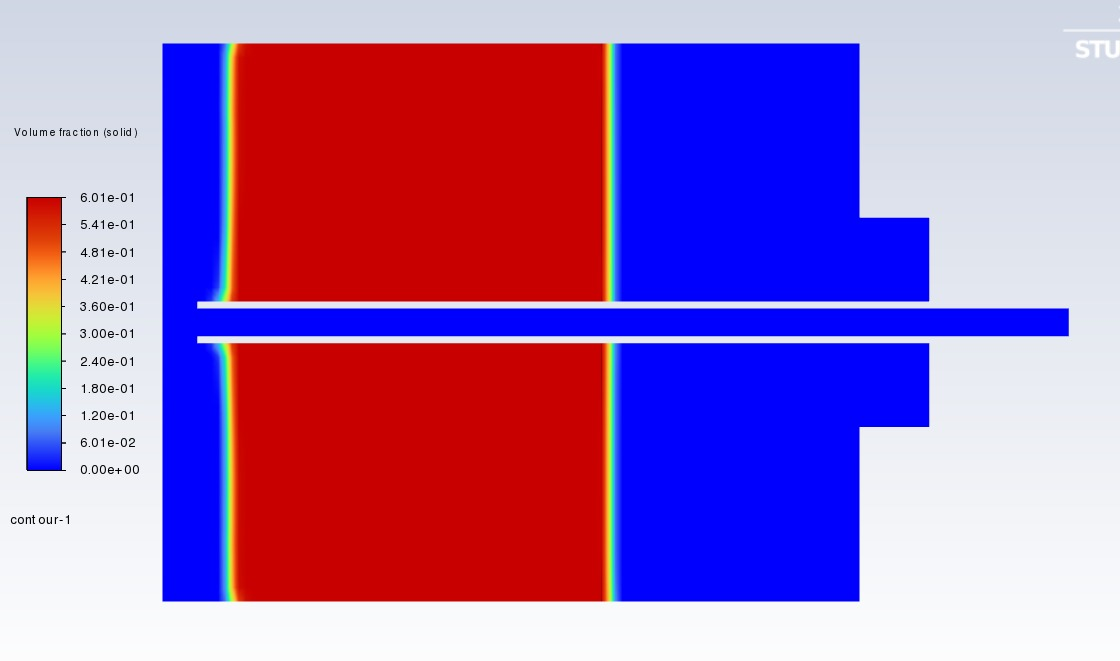
\includegraphics[width=\textwidth]{../report_assets/no_grav.png}
        \caption*{(b) Under Microgravity}
    \end{minipage}
    \caption{Phase Density of Old Design after 2 Seconds}
\end{figure}

\begin{figure}[htbp]
    \centering

    \begin{minipage}{0.45\textwidth}
        \centering
        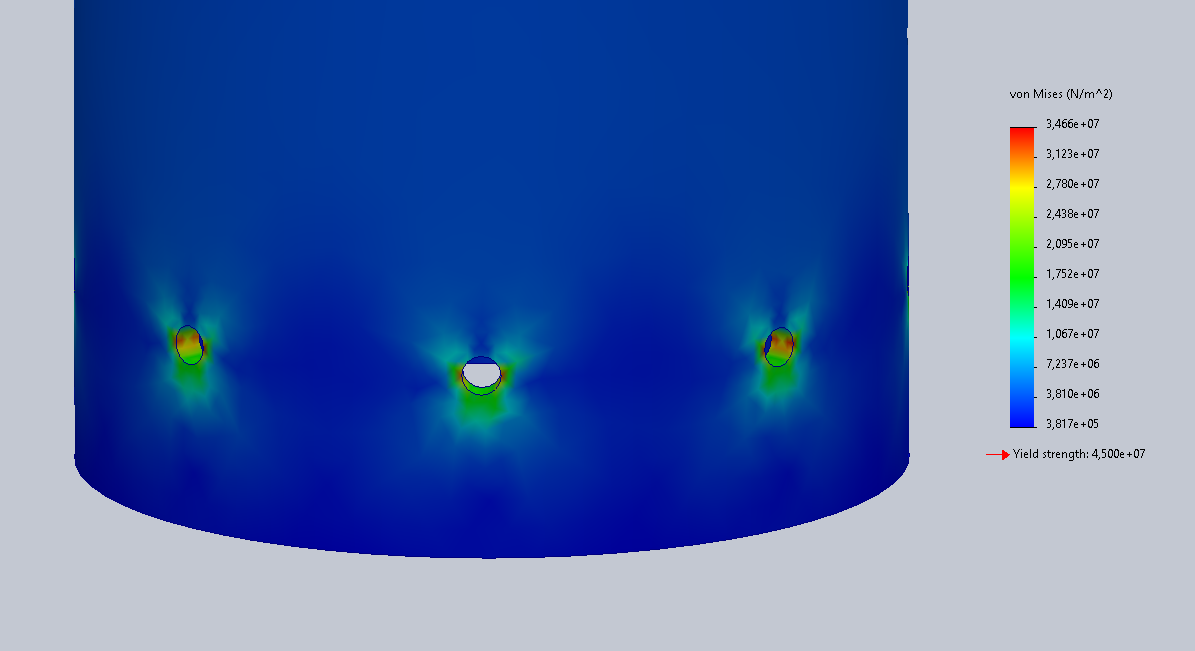
\includegraphics[width=\textwidth]{../report_assets/unprocessed_fea_fine.png}
        \caption*{(a) Fine Mesh}
    \end{minipage}    
    \hfill
    \begin{minipage}{0.45\textwidth}
        \centering
        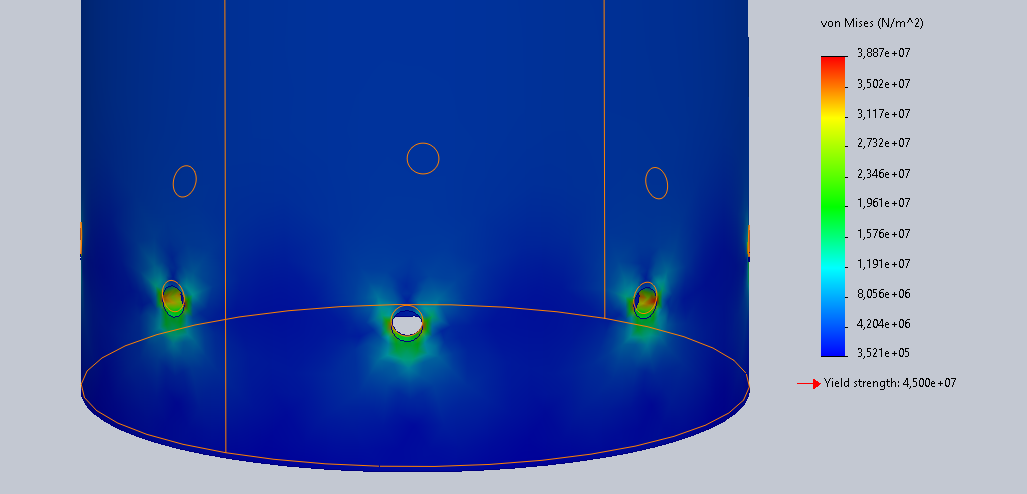
\includegraphics[width=\textwidth]{../report_assets/unprocessed_fea_coarse.png}
        \caption*{(b) More Coarse Mesh}
    \end{minipage}    
    \caption{Results of Tank FEA}

\end{figure}  

\begin{figure}[htbp]
    \centering

    \begin{minipage}{0.8\textwidth}
        \centering
        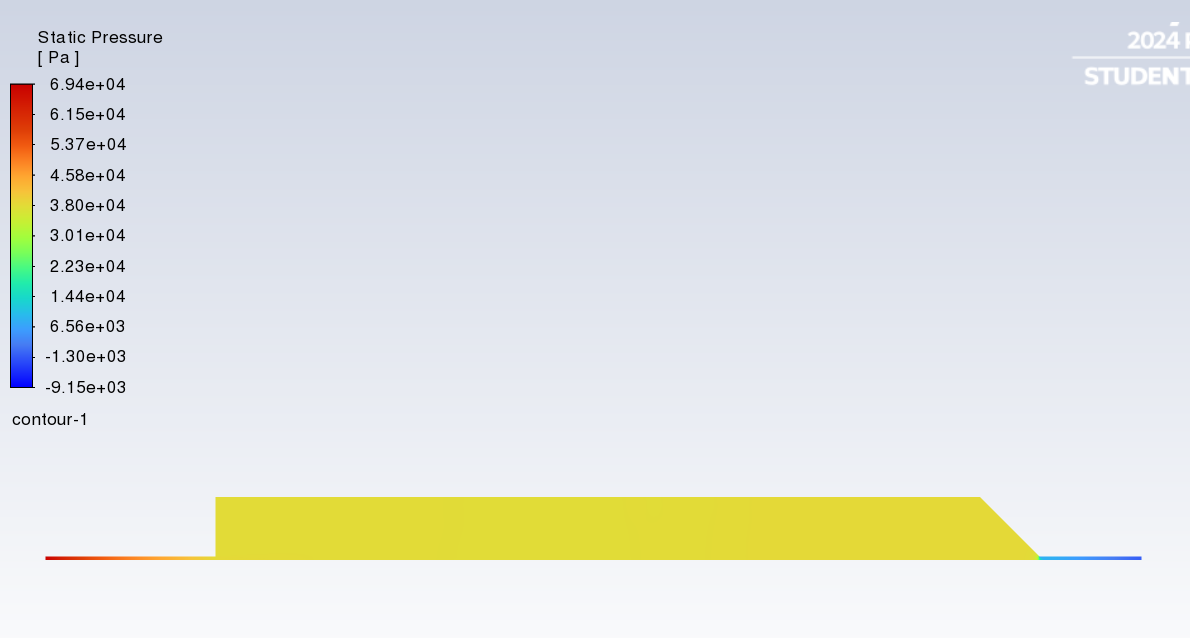
\includegraphics[width=\textwidth]{../report_assets/unprovessed_stat_pres.png}
        \caption{Static Pressure of Empty Tank Simulation}
    \end{minipage}    
\end{figure}  

\begin{figure}[htbp]
    \centering
    \begin{minipage}{0.8\textwidth}
        \centering
        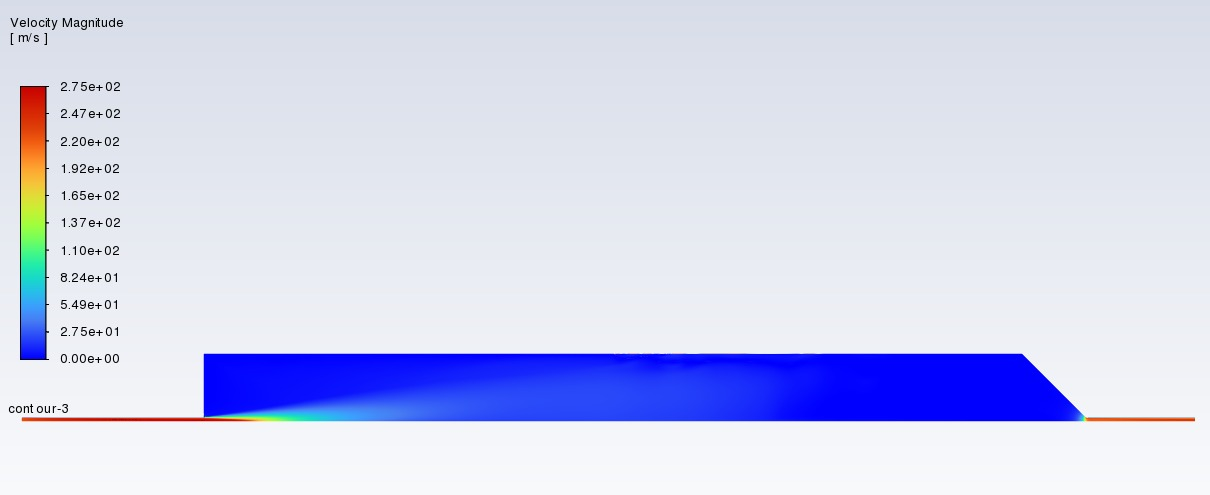
\includegraphics[width=\textwidth]{../report_assets/unprovessed_vel.jpeg}
        \caption{Velocity Magnitude of Empty Tank Simulation}
    \end{minipage}    
\end{figure}  

\chapter{End Cap Engineering Drawings}

\begin{figure}[htbp]
    \centering
    \begin{minipage}{0.8\textwidth}
        \centering
        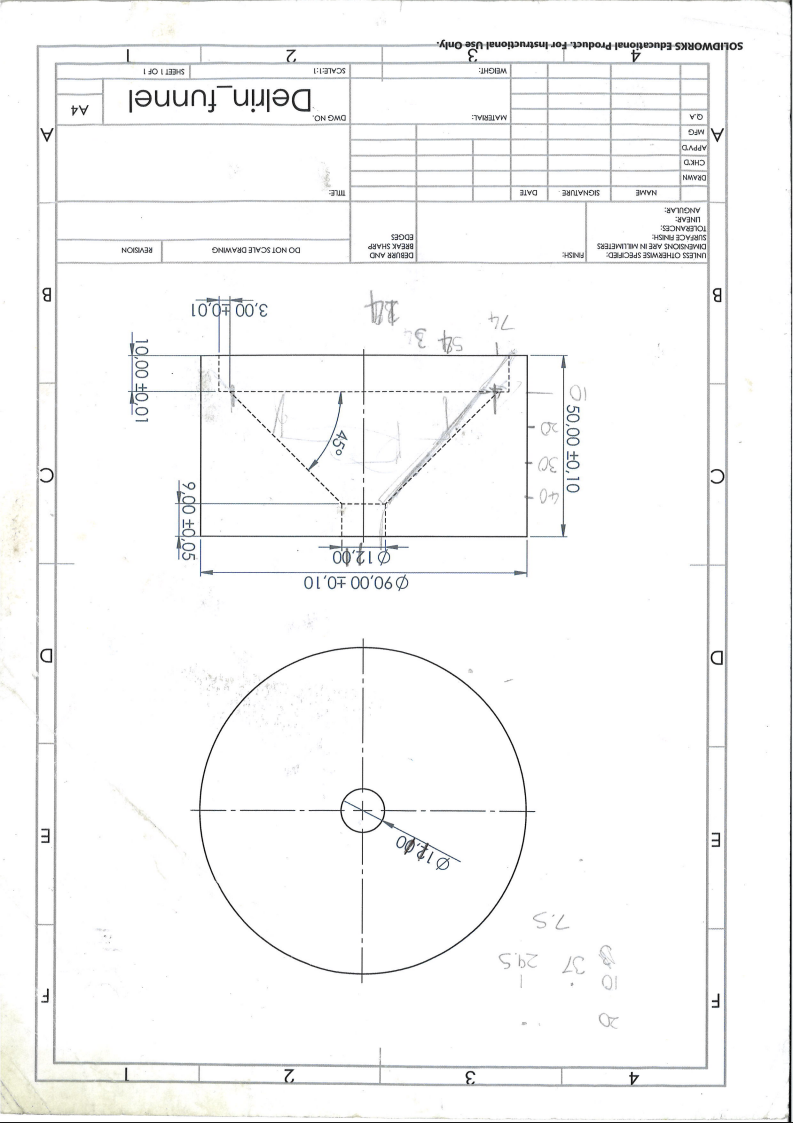
\includegraphics[width=\textwidth, angle=180]{../report_assets/funnel_eng_draw.png}
        \caption{Outlet End Cap Engineering Drawing}
    \end{minipage}    
\end{figure}  

\begin{figure}[htbp]
    \centering
    \begin{minipage}{0.8\textwidth}
        \centering
        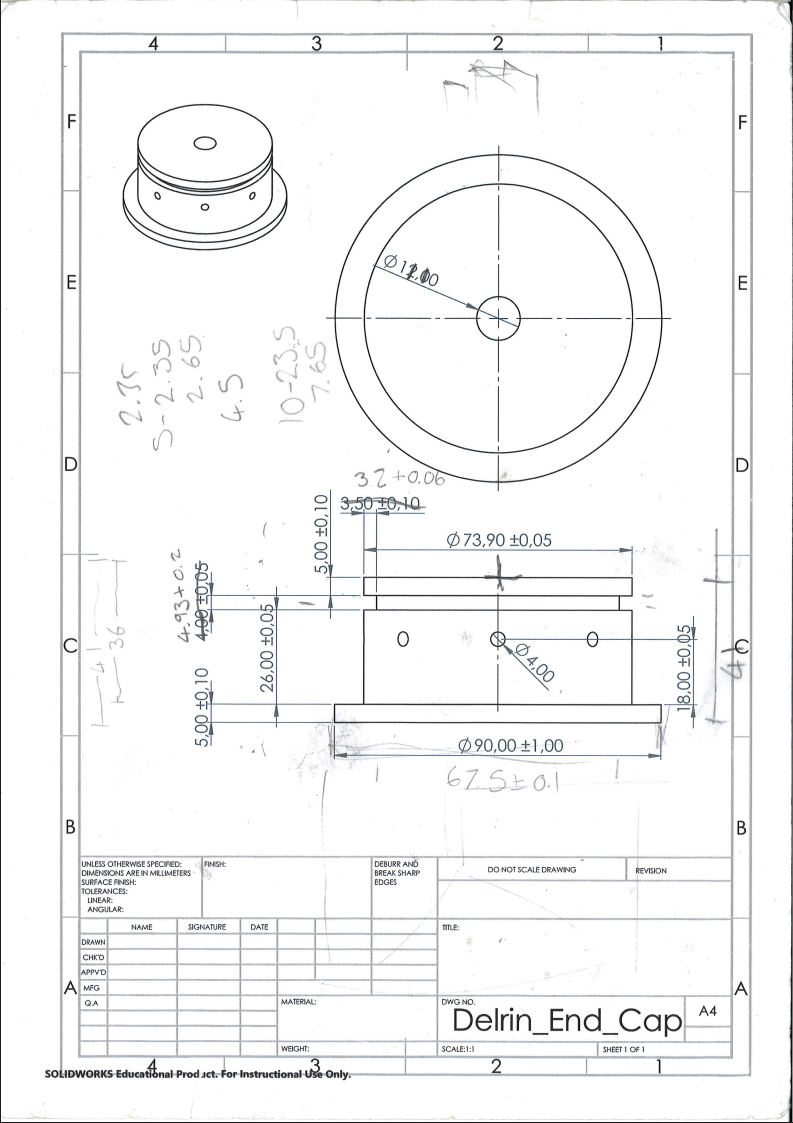
\includegraphics[width=\textwidth]{../report_assets/end_cap_eng_draw.png}
        \caption{Inlet End Cap Engineering Drawing}
    \end{minipage}    
\end{figure}  

\chapter{Mass Flow Analysis Code}

\begin{lstlisting}[language=Python, caption={Example Python code for Mass Flow Analysis}]
import matplotlib.pyplot as plt
import pandas as pd

# Read the CSV files
input_file_1 = 'Research_Files/June/5_bar_sand/2_kermit106.csv'  # 0 2 7
input_file_2 = 'Research_Files/June/5_bar_sand/2_kermit108.csv'  # 0 1 7

# Load the data into a DataFrame
df_1 = pd.read_csv(input_file_1)
df_2 = pd.read_csv(input_file_2)

# Keep only the specified columns
df_1 = df_1[['BackendTime', 'ch0sens', 'ch2sens', 'ch7sens']]
df_2 = df_2[['BackendTime', 'ch0sens', 'ch1sens', 'ch7sens']]

# Rescale BackendTime to seconds and set the first value to 0
df_1['BackendTime'] = (df_1['BackendTime'] - 1748808369580) / 1e3
df_2['BackendTime'] = (df_2['BackendTime'] - 1748808369580) / 1e3

df_1 = df_1[(df_1['BackendTime'] >= 33) & (df_1['BackendTime'] <= 82)]
df_2 = df_2[(df_2['BackendTime'] >= 33) & (df_2['BackendTime'] <= 82)]

plt.rc('legend', fontsize=24)   # Increase legend font size
plt.rc('lines', linewidth=4)    # Further increase line width
plt.rc('axes', labelsize=28)    # Increase axis label font size
plt.figure(figsize=(12, 8))    # Increase figure size
plt.rc('xtick', labelsize=24)   # Increase x-axis tick font size
plt.rc('ytick', labelsize=24)   # Increase y-axis tick font size
# plt.plot(df_1['BackendTime'], df_1['ch0sens'], label='Inlet PT (df_1)') ### used to determine the opening and closing of the valves
plt.plot(df_1['BackendTime'], df_1['ch2sens'], label='Start of Tank', color='blue')
plt.plot(df_1['BackendTime'], df_1['ch7sens'], label='End of Tank', color='red')
plt.plot(df_2['BackendTime'], df_2['ch7sens'], label='Cyclone Seperator', color='orange')
plt.axvline(x=39.5, color='green', linestyle='--')
plt.axvline(x=74.9, color='green', linestyle='--')
# Remove all values before 8 seconds
# Add labels and title
plt.xlabel('Experiment Time (s)')
plt.ylabel('Load Cell Values (kg)')
plt.ylim(0.1, 2.1)
plt.legend()
plt.tight_layout()
# Show the plot
plt.savefig('./latex/report_assets/52_raw_mass.png')
df_1['ch2plus7'] = df_1['ch2sens'] + df_1['ch7sens']
# Save cleaned DataFrames to new CSV files
df_1.to_csv(input_file_1.replace('.csv', '_clean.csv'), index=False)
df_2.to_csv(input_file_2.replace('.csv', '_clean.csv'), index=False)


# import matplotlib.pyplot as plt
# import pandas as pd

# # Read the CSV files
# input_file_1 = 'Research_Files/June/5_bar_sand/2_kermit106_clean.csv'  # 0 2 7
# input_file_2 = 'Research_Files/June/5_bar_sand/2_kermit108_clean.csv'  # 0 1 7

# # Load the data into a DataFrame
# df_1 = pd.read_csv(input_file_1)
# df_2 = pd.read_csv(input_file_2)

# # Keep only the specified columns
# df_1 = df_1[['BackendTime', 'ch0sens', 'ch2sens', 'ch2plus7']]
# df_2 = df_2[['BackendTime', 'ch0sens', 'ch1sens', 'ch7sens']]


# plt.rc('legend', fontsize=24)   # Increase legend font size
# plt.rc('lines', linewidth=4)    # Further increase line width
# plt.rc('axes', labelsize=28)    # Increase axis label font size
# plt.figure(figsize=(12, 8))    # Increase figure size
# plt.rc('xtick', labelsize=24)   # Increase x-axis tick font size
# plt.rc('ytick', labelsize=24)   # Increase y-axis tick font size

# plt.plot(df_1['BackendTime'], df_1['ch2plus7'], label='Combined Tank', color='purple')
# plt.plot(df_2['BackendTime'], df_2['ch7sens'], label='Cyclone Seperator', color='orange')

# plt.axvline(x=39.5, color='green', linestyle='--')
# plt.axvline(x=74.9, color='green', linestyle='--')
# # Add labels and title
# plt.xlabel('Experiment Time (s)')
# plt.ylabel('Load Cell Values (kg)')
# plt.legend()
# plt.tight_layout()
# # plt.show()
# # # Show the plot
# plt.savefig('./latex/report_assets/52_clean_mass.png')


# import matplotlib.pyplot as plt
# import pandas as pd

# # Read the CSV files
# input_file_1 = 'Research_Files/June/5_bar_sand/2_kermit106_clean.csv'  # 0 2 7
# input_file_2 = 'Research_Files/June/5_bar_sand/2_kermit108_clean.csv'  # 0 1 7

# # Load the data into a DataFrame
# df_1 = pd.read_csv(input_file_1)
# df_2 = pd.read_csv(input_file_2)

# df_1 = df_1[['BackendTime', 'ch0sens', 'ch2sens', 'ch2plus7']]
# df_2 = df_2[['BackendTime', 'ch0sens', 'ch1sens', 'ch7sens']]

# df_1['ch2plus7'] = -1*df_1['ch2plus7']
# df_1['m_flow'] = df_1['ch2plus7'].diff()
# df_2['m_flow'] = df_2['ch7sens'].diff()
# # Apply a rolling mean to smooth the curves
# window_size = 100  # Adjust as needed for smoothing
# df_1['smooth_combined'] = df_1['ch2plus7'].rolling(window=window_size, center=True, min_periods=1).mean()
# df_2['smooth_ch7sens'] = df_2['ch7sens'].rolling(window=window_size, center=True, min_periods=1).mean()

# df_1['m_flow_smooth'] = df_1['smooth_combined'].diff()*10
# df_2['m_flow_smooth'] = df_2['smooth_ch7sens'].diff()*10

# plt.rc('legend', fontsize=24)   # Increase legend font size
# plt.rc('lines', linewidth=4)    # Further increase line width
# plt.rc('axes', labelsize=28)    # Increase axis label font size
# plt.figure(figsize=(12, 8))    # Increase figure size
# plt.rc('xtick', labelsize=24)   # Increase x-axis tick font size
# plt.rc('ytick', labelsize=24)   # Increase y-axis tick font size

# plt.plot(df_1['BackendTime'], df_1['m_flow_smooth']*1000, label='Combined Tank', color='purple')
# plt.plot(df_2['BackendTime'], df_2['m_flow_smooth']*1000, label='Cyclone Seperator', color='orange')

# plt.axvline(x=39.5, color='green', linestyle='--')
# plt.axvline(x=49.5, color='red', linestyle='--')
# plt.axvline(x=59.9, color='red', linestyle='--')
# plt.axvline(x=74.9, color='green', linestyle='--')

# plt.xlabel('Experiment Time (s)')
# plt.ylabel('Mass Flow Rate (g/s)')
# plt.ylim(-10, 52)
# plt.legend(loc='lower center')
# plt.tight_layout()
# # # Show the plot
# plt.savefig('./latex/report_assets/52_clean_flow_100.png')

\end{lstlisting}

As you can most-likely tell, some of this code was written with the help of ChatGPT.\@